                \section{Restauration (Inpainting)}
  Problem: Lücken im Bild, etwa

  \begin{enumerate}
    \item Kratzer
    \item Scannerzeile kaputt
    \item Defekt in der Kamera
    \item Bewusst entferntes Objekt
  \end{enumerate}
  sollen sinnvoll und unauffällig geschlossen werden.

  Sei $f: \Omega \to F$ unser Bild jedoch mit Defekt, d.h. fehlenden Funktionswerten in $D \subset \Omega$.

  \begin{enumerate}
    \item[1. Fall:] Jeder Punkt aus $D$ hat Nachbarn in $\Omega \backslash D$.\\
    $\Rightarrow$ Lücken mittels Interpolation aus benachbarten Werten in $\Omega \backslash D$ schließen.
    \item[2. Fall:] $D$ hat innere Punkte. Diesen Fall werden wir im folgenden näher betrachten.
  \end{enumerate}

  \subsection{Frequenzraum-Ansatz}
    Zur Illustration in 1D:
    \begin{center}
      \begin{tikzpicture}[scale = 1.3]
        \draw (0,0) -- (8,0);
        \draw[thick] plot [smooth, tension = 0.8] coordinates {(1,1) (2,1.2) (3,1) (4,1.3) (5,1.7) (6,1.5) (7,2)};
        \draw[fill,color=white] (3,0.5) rectangle (5,2);
        \draw (1,-0.1) -- (1,0.1);
        \draw (3,-0.1) -- (3,0.1);
        \draw (5,-0.1) -- (5,0.1);
        \draw (7,-0.1) -- (7,0.1);
        \draw (5.3,-0.1) -- (5.3,0.1);
        \draw (2.7,-0.1) -- (2.7,0.1);
        \draw[decorate,decoration={brace,amplitude=2pt,mirror}] (1,-0.5) -- node[below] {\small $\Omega$} (7,-0.5);
        \draw[thick, line width =0.6mm] (3,0) -- node[below] {\small $D$} (5,0);
        \draw[decorate,decoration={brace,amplitude=2pt,mirror}] (2.7,-0.15) -- node[below] {\small $u$} (3,-0.15);
        \draw[decorate,decoration={brace,amplitude=2pt,mirror}] (5,-0.15) -- node[below] {\small $u$} (5.3,-0.15);
      \end{tikzpicture}
    \end{center}
    Betrachte Umgebung $u \subset \Omega \backslash D$ und errechne den Mittelwert:
    \[ m \coloneqq  \frac{1}{\abs{u}} \int_u f(x) dx\]
    von $f$ auf $u$.

    \textbf{Algorithmus:}

    \begin{tikzpicture}
        \node at (5, 10) {
    {\begin{varwidth}{\linewidth}\begin{enumerate}[label=]
        \item[\texttt{[1]}] Initialisiere $f$ auf $D$ mittels konstanter Funktion $m$:
          \begin{center}
            \begin{tikzpicture}
              \draw (0,0) -- (8,0);
              \draw[thick] plot [smooth, tension = 0.8] coordinates {(1,1) (2,1.2) (3,1) (4,1.3) (5,1.7) (6,1.5) (7,2)};
              \draw[fill,color=white] (3,0.5) rectangle (5,2);
              \draw (1,-0.1) -- (1,0.1);
              \draw (3,-0.1) -- (3,0.1);
              \draw (5,-0.1) -- (5,0.1);
              \draw (7,-0.1) -- (7,0.1);
              \draw[dashed,thick,red,line width=0.4mm] (3,1) -- (3,1.4) -- (5,1.4) -- (5,1.7);
              \draw[thick, line width =0.6mm] (3,0) -- node[below] {\small $D$} (5,0);
              \draw[<-] (3.05,1.2) -- (6,0.5);
              \draw[<-] (5.05,1.6) -- (6,0.5) node[right] {\small Sprünge};
            \end{tikzpicture}
          \end{center}
          $\Rightarrow$ Sprünge am Rand von $D$.\\
          Idee: Sprünge $\widehat =$ hochfrequente Anteile $\Rightarrow$ wende Tiefpass filter an.
        \item[\texttt{[2]}] $ f \xrightarrow{\F} \hat f \xrightarrow{\text{Lösche hohe Frequenzen}} \hat g \xrightarrow{\F^{-1}}g$
          \begin{center}
            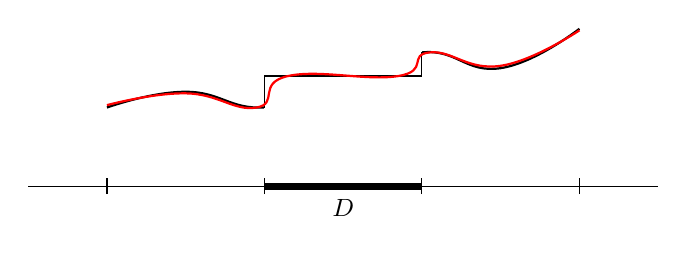
\begin{tikzpicture}
              \draw (0,0) -- (8,0);
              \draw[thick] plot [smooth, tension = 0.8] coordinates {(1,1) (2,1.2) (3,1) (4,1.3) (5,1.7) (6,1.5) (7,2)};
              \draw[fill,color=white] (3,0.5) rectangle (5,2);
              \draw (1,-0.1) -- (1,0.1);
              \draw (3,-0.1) -- (3,0.1);
              \draw (5,-0.1) -- (5,0.1);
              \draw (7,-0.1) -- (7,0.1);
              \draw[] (3,1) -- (3,1.4) -- (5,1.4) -- (5,1.7);
              \draw[thick, line width =0.9mm] (3,0) -- node[below] {\small $D$} (5,0);
              \draw[thick,red] plot [smooth, tension = 0.8] coordinates {(1,1.03) (2,1.18) (2.9,1) (3.3,1.4) (4.7,1.4) (5.1,1.7) (6,1.53) (7,1.98)};
            \end{tikzpicture}
          \end{center}
        \item[\texttt{[3]}] Ersetze $f$ \underline{innerhalb} von $D$ durch $g$.
          \begin{center}
            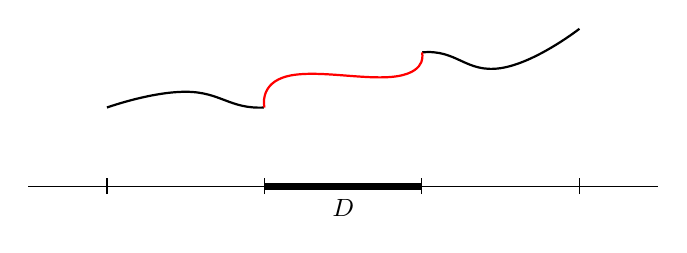
\begin{tikzpicture}
              \draw (0,0) -- (8,0);
              \draw[thick] plot [smooth, tension = 0.8] coordinates {(1,1) (2,1.2) (3,1) (4,1.3) (5,1.7) (6,1.5) (7,2)};
              \draw[fill,color=white] (3,0.5) rectangle (5,2);
              \draw (1,-0.1) -- (1,0.1);
              \draw (3,-0.1) -- (3,0.1);
              \draw (5,-0.1) -- (5,0.1);
              \draw (7,-0.1) -- (7,0.1);
              \draw[thick, line width =0.9mm] (3,0) -- node[below] {\small $D$} (5,0);
              \draw[thick,red] plot [smooth, tension = 0.8] coordinates {(3,1) (3.3,1.4) (4.7,1.4) (5,1.7)};
            \end{tikzpicture}
          \end{center}
      \end{enumerate}\end{varwidth}}};
      \draw[->,thick] (0,5.5) -- (-1,5.5) -- node[sloped,above]  {Iteriere} node[sloped,below] {\footnotesize Abbruch falls $\norm{f-g}<$ threshold} (-1,10.9) -- (-0.5,10.9);
    \end{tikzpicture}

  \subsection{PDE-Transport-Diffusions-Ansatz}
    \begin{minipage}[c]{0.25\linewidth}
      \begin{center}
        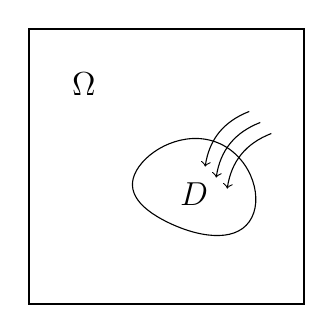
\begin{tikzpicture}[scale=0.7]
          \draw[thick] (0,0) rectangle (5,5);
          \draw plot [smooth cycle,tension=1] coordinates {(2.5,1.5) (2,2.5) (3.5,2.9) (4,1.5)};
          \draw (3,2) node[] {\large $D$};
          \draw (1,4) node[] {\large $\Omega$};
          \draw[<-] (3.2,2.5) to[bend left] (4,3.5);
          \draw[<-] (3.4,2.3) to[bend left] (4.2,3.3);
          \draw[<-] (3.6,2.1) to[bend left] (4.4,3.1);
        \end{tikzpicture}
      \end{center}
    \end{minipage}
    \hfill
    \begin{minipage}[c]{0.65\linewidth}
        \begin{enumerate}
          \item[Idee:] Informationen aus $\Omega \backslash D$ nach $D$ ''hineinragen''.
          \item[Referenzen:] \begin{enumerate}
            \item[\textbullet] Weichert 1998
            \item[\textbullet] Bornemann \& März 2007
          \end{enumerate}
        \end{enumerate}
    \end{minipage}
    \ \\
    \ \\
    \hfill\\
    \textbf{Skalierung der Diffusion:}
    \[\frac{\partial u}{\partial t} = div(M \nabla u)\]
    \[\text{mit } M = \srmatrix{ | & |\\ v_1 & v_2\\ | & |} \mat{\lambda_1 & \ \\ & \lambda_2} \srmatrix{- & v_1^T & -\\ \\- & v_2^T & -} \in \R^{2 \times 2}\]
    Wobei $v_1 \perp v_2$ die Eigenvektoren des sogenannten \underline{doppelt geglätteten Strukturtensors} \index{doppelt geglätteter Strukturtensor}
    \[J= G_\rho * \biggl[ \underbrace{\srmatrix{| \\ \nabla (G_\sigma * u)\\ |}}_{2 \times 1} \cdot \underbrace{\srmatrix{- & \nabla^T(G_\sigma * u) & -}}_{1 \times 2} \biggr] \]
    sind.\\
    \begin{enumerate}
      \item[$\Rightarrow$] $v_1$ Richtung mit maximalem Kontrast mit EW $\mu_1$
      \item[] $v_2$ Richtung mit minimalem Kontrast mit EW $\mu_2$, genannt \mim{Kohärentsrichtung}.
      \item[] Hierbei ist $\mu_1 \geq \mu_2$.
    \end{enumerate}

    \begin{center}
        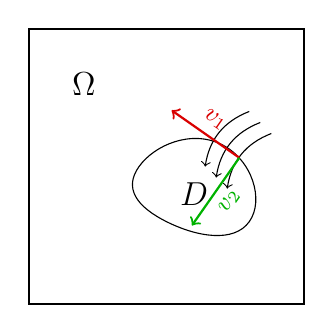
\begin{tikzpicture}[scale=0.7]
          \draw[thick] (0,0) rectangle (5,5);
          \draw plot [smooth cycle,tension=1] coordinates {(2.5,1.5) (2,2.5) (3.5,2.9) (4,1.5)};
          \draw (3,2) node[] {\large $D$};
          \draw (1,4) node[] {\large $\Omega$};
          \draw[<-] (3.2,2.5) to[bend left] (4,3.5);
          \draw[<-] (3.4,2.3) to[bend left] (4.2,3.3);
          \draw[<-] (3.6,2.1) to[bend left] (4.4,3.1);
          \draw[->,red!85!black,thick] (3.82,2.66) -- node[sloped,above] {\small $v_1$} ++(-215:1.5);
          \draw[->,green!70!black,thick] (3.82,2.66) -- node[sloped,below] {\small $v_2$} ++(-125:1.5);
        \end{tikzpicture}
      \end{center}

      Fälle:
      \begin{enumerate}
        \item[]
        \begin{minipage}[c]{0.25\linewidth}
          $\mu_1 \gg \mu_2 \approx 0$
        \end{minipage}
        \begin{minipage}[c]{0.25\linewidth}
          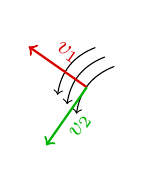
\begin{tikzpicture}[scale =0.6]
            \draw[<-] (3.2,2.5) to[bend left] (4,3.5);
            \draw[<-] (3.4,2.3) to[bend left] (4.2,3.3);
            \draw[<-] (3.6,2.1) to[bend left] (4.4,3.1);
            \draw[->,red!85!black,thick] (3.82,2.66) -- node[sloped,above] {\small $v_1$} ++(-215:1.5);
          \draw[->,green!70!black,thick] (3.82,2.66) -- node[sloped,below] {\small $v_2$} ++(-125:1.5);
          \end{tikzpicture}
        \end{minipage}
                \item[]
        \begin{minipage}[c]{0.25\linewidth}
          $\mu_1 \approx \mu_2 \approx 0$
        \end{minipage}
        \begin{minipage}[c]{0.12\linewidth}
          
\begin{tikzpicture}[scale =0.6]
            \definecolor{left} {HTML}{001528}
            \draw[shading = axis,rectangle, left color=left!70!white, right color=left!60!white,shading angle=135, anchor=north,fill,draw=white] (0,0) rectangle (2,2);
          \end{tikzpicture}
        \end{minipage}
        \begin{minipage}[c]{0.3\linewidth}
          Lokal keine Struktur.
        \end{minipage}
        \item[]
        \begin{minipage}[c]{0.25\linewidth}
          $\mu_1 \approx \mu_2 \gg 0$
        \end{minipage}
        \begin{minipage}[c]{0.12\linewidth}
          
\begin{tikzpicture}[scale =0.6]
            \definecolor{left} {HTML}{001528}
            \draw[shading = axis,rectangle, left color=left!20!white, right color=left!30!white,shading angle=135, anchor=north,fill,draw=white] (0,0) rectangle (2,2);
            \draw[line width = 0.8mm] (0,0) -- (2,0) -- (2,2);
          \end{tikzpicture}
        \end{minipage}
        \begin{minipage}[c]{0.3\linewidth}
          Kanten.
        \end{minipage}
      \end{enumerate}

      Die Werte $\lambda_1$ und $\lambda_2$ werden wie folgt gewählt:\\
      $\alpha \in (0,1)$ wird festgehalten.

      \begin{center}
        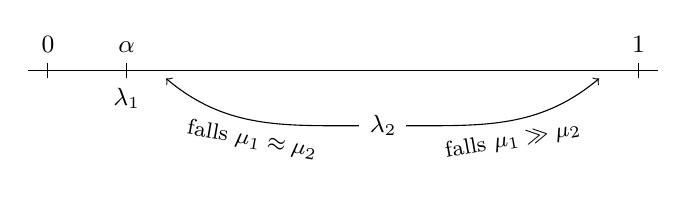
\begin{tikzpicture}[scale = 1]
            \draw[] (0,0) -- (8,0);
            \draw (0.25,-0.1) -- (0.25,0.1) node[above] {\small $0$};
            \draw (7.75,-0.1) -- (7.75,0.1) node[above] {\small $1$};
            \draw (1.25,-0.1) node[below] {\small $\lambda_1$} -- (1.25,0.1) node[above] {\small $\alpha$};
            \draw[->] (4.2,-0.7) to[out=180, in =-40] node[sloped,below] {\footnotesize falls $\mu_1 \approx \mu_2$} (1.75,-0.1);
            \draw[<-] (7.25,-0.1) to[in=0,out =-140] node[sloped,below] {\footnotesize falls $\mu_1 \gg \mu_2$} (4.8,-0.7) node[left] {\small $\lambda_2$};
          \end{tikzpicture}
      \end{center}

      \[\lambda_1  \coloneqq  \alpha, \ \lambda_2  \coloneqq  \alpha + (1 - \alpha)(1-g(\mu_1 - \mu_2))\]

      wobei $g$ wie bei Perona Malik gewählt wird, also:

      \[g(x)=\frac{1}{1 + \frac{s^2}{\kappa^2}}\]

      Dieses wird \mim{Kohärenz verstärkende Diffusion} genannt.

      \subsection{Variationsansatz}


      \begin{minipage}[c]{0.5\linewidth}
        \begin{enumerate}
          \item[geg.:] $f$ auf $\Omega \backslash D$
          \item[ges.:] $u$ auf $\Omega$
          \item[Wunsch 1:] $u=f$ auf $\Omega \backslash D$
          \item[Wunsch 2:] $\norm{\nabla u}$ klein auf $\Omega$
        \end{enumerate}
    \end{minipage}
    \hfill
    \begin{minipage}[c]{0.35\linewidth}
      \begin{center}
        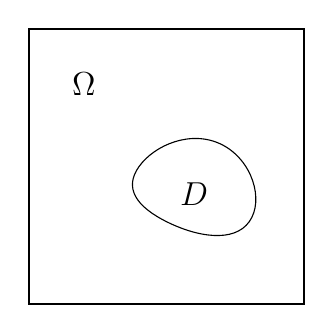
\begin{tikzpicture}[scale=0.7]
          \draw[thick] (0,0) rectangle (5,5);
          \draw plot [smooth cycle,tension=1] coordinates {(2.5,1.5) (2,2.5) (3.5,2.9) (4,1.5)};
          \draw (3,2) node[] {\large $D$};
          \draw (1,4) node[] {\large $\Omega$};
        \end{tikzpicture}
      \end{center}
    \end{minipage}\\
    \hfill\\ \hfill\\
    Daraus folgt:

    \[ J(u) \coloneqq  \norm{\nabla u}_2^2 \to \text{min} \]

    auf

    \[U \coloneqq \{u \in W^{1,2}(\Omega) : u|_{\Omega \backslash D} = f\} \]

    Angenommen, $u \in U$ minimiert $J$, dann folgt für beliebige $v \in W^{1,2} (\Omega)$ mit $v|_{\Omega \backslash D}=0$:

    \begin{align*}
      0 &= \underset{t \to 0}{lim} \frac{J(u+tv) - J(u)}{t} = \underset{t \to 0}{lim} \frac{1}{t} \int_\Omega ||\underbrace{\nabla(u+tv)(x)}_{\nabla u(x) + t \nabla v(x)}||^2 - \norm{\nabla u(x)}^2 dx\\
      &=\underset{t \to 0}{lim} \frac{1}{t} \int_\Omega \skprod{\nabla u(x) + t \nabla v(x)}{\nabla u(x) + t \nabla v(x)} - \skprod{\nabla u (x)}{\nabla u (x)} dx\\
      &=\underset{t \to 0}{lim} \frac{1}{t} \int_\Omega t^2 \norm{\nabla v(x)}^2 + 2 t \skprod{\nabla u(x)}{\nabla v(x)} dx =  \underset{t \to 0}{lim} \int_\Omega t \norm{\nabla v(x)}^2 + 2 \skprod{\nabla u(x)}{\nabla v(x)} dx\\
      &=2 \int_D \skprod{\nabla u(x)}{\nabla v(x)} dx \overset{\text{Greensche Formel}}{=} 2 \biggl( \overbrace{\int_{\delta D} \frac{\partial u}{\partial n} \underbrace{v(x)}_{0} ds(x)}^{0} - \int_D \Delta u(x) v(x) dx \biggr)\\
      &=2 \int_D \Delta u(x) v(x) dx \Rightarrow \Delta u =0 \text{ in } D
    \end{align*}

